\documentclass[12pt]{article}

\input{../../Latex_Common/skinnerr_latex_preamble_asen5417.tex}

%%
%% DOCUMENT START
%%

\begin{document}

\pagestyle{fancyplain}
\lhead{}
\chead{}
\rhead{}
\lfoot{ASEN 5417: Homework 1}
\cfoot{\thepage}
\rfoot{Ryan Skinner}

\noindent
{\Large Homework 1}
\hfill
{\large Ryan Skinner}
\\[0.5ex]
{\large ASEN 5417: Numerical Methods}
\hfill
{\large Due 2015/09/08}\\
\hrule
\vspace{12pt}

\section{Introduction}

When integrating functions of one or more variables, analytic solutions are desired because they offer a complete description of solution behavior. For most situations of engineering interest, however, the governing equations defy all attempts to obtain a closed solution. In such instances, numerical integration provides a tool for exploring the solution space.

We solve the following problems to better understand the tools of numerical integration. As will be described in the methods section, our tools include the trapezoidal method, Simpson's method, and Richardson extrapolation.

\subsection{Problem A}

We wish to show that the equality
\begin{equation}
\int_{0}^{2\pi} \frac{dx}{1 + a \cos x} = \frac{2\pi}{\sqrt{1-a^2}}, \qquad a^2 < 1
\label{eq:a}
\end{equation}
holds for $a = \tfrac{1}{2}$. This is a relatively simple finite integral of a continuous function with no singularities.

\subsection{Problem B}

We wish to confirm the equalities
\begin{equation}
\text{(i)} \quad
\int_{0}^{\infty} \frac{\sin^4 x}{x^4} \; dx = \frac{\pi}{3}
,
\qquad
\text{and}
\qquad
\text{(ii)} \quad
\int_{0}^{\infty} \frac{\sin x}{\sqrt{x}} \; dx = \sqrt{\frac{\pi}{2}}
.
\label{eq:b}
\end{equation}
Note that both integrands are indeterminate at $x=0$ and otherwise periodic, and that both integrals extend indefinitely. Particular care will need to be paid to singularities, periodicity, and limits of integration.

\subsection{Problem C}

Moving to functions of two variables, we wish to estimate
\begin{equation}
I = \int_1^3 \int_1^2 f(x,y) \; dx \; dy
\end{equation}
for the integrands
\begin{equation}
\text{(i)} \quad
f(x,y) = x y (1+x)
,
\qquad
\text{and}
\qquad
\text{(ii)} \quad
f(x,y) = x^2 y^3 (1+x)
.
\label{eq:c}
\end{equation}
As in the first problem, these expressions involve well-behaved integrands and finite bounds. Application of our chosen numerical method over a two-dimensional domain will be the crux of this problem.

\section{Methodology}

Versions of the trapezoidal method, Simpson's method, and Richardson extrapolation are all implemented in \textsc{Matlab}. The following problems employ a subset of these methods in their solution.

The value of $\pi$ used for calculations is always obtained through the equality $\pi = 4 \arctan(1)$.

\subsection{Problem A}

To solve this problem, we use Simpson's method with $N_1=\{10,20\}$ and $N_2=\{100,200\}$ equally-spaced parts. That is, we split the interval $x \in [0,2\pi]$ with equally spaced points $x_i, i \in [0,N]$ such that $x_0 = 0$ and $x_N = 2\pi$. In all cases, we calculate the relative error as
\begin{equation}
e_r = \frac{\left| f_e - f_c \right|}{f_e}
,
\end{equation}
where $f_e$ is the exact value of the integral and $f_c$ is the computed value. We then apply Richardson extrapolation to the sets $N_1$ and $N_2$, to see if it improves our estimate $f_c$.

\subsection{Problem B}

Recall that three topics must be addressed in this problem:
\begin{enumerate}
\item Singular integrand at $x=0$
\item Periodicity
\item Indefinite limit of integration
\end{enumerate}

To address the singularities at $x=0$, we Taylor-expand $\sin x$ about $x=0$, to arrive at $\sin x \approx x + \bigo(x^2)$. Keeping only first-order terms in the limit as $x \rightarrow 0$, we substitute $\sin x \approx x$ into the integrands in \eqref{eq:b}. Thus the respective integrands are equal to $1$ and $0$ as $x \rightarrow 0$. By using these limiting values when evaluating the integrands at $x=0$, singularities are addressed.

Periodicity is coupled with choosing a finite limit for the indefinite integral. Both are addressed as follows.

For \eqref{eq:b}(i), periodicity is not very important, since we know $\sin^4 x$ is bounded by $[0,1]$, and the integrand drops off in magnitude with $x^4$. Nonetheless, we truncate the indefinite integral at $x=8\pi$, where the last period has a maximum at $x = 7.5 \pi$ of $\sim 3.2 \times 10^{-6}$ (nearly 6 orders of magnitude lower than the first maximum at $x=\pi/2$).

For \eqref{eq:a}(ii), we note that $\sin x$ has a range of $[-1,1]$ over each period. It is thus advantageous to numerical accuracy to truncate our integration at some multiple of $2\pi$. If the similar-magnitude positive and negative parts of each period are both accounted for, any ``incomplete'' period at the end of our interval could sway the resulting integral disproportionately. After some experimentation, the maximum bound on integration was set to $600 \pi$. The bound is so far out because the integrand decays very slowly, proportional to $x^{1/2}$.

\subsection{Problem C}

For these integrals, we perform integration once in the $x$-direction and once in the $y$-direction. We use $h = dx = \tfrac{1}{2}$, and $k = dy = 1$. This means we have nine grid points in our domain, and use Simpson's method on one slab of width $2h$ and $2k$ in each direction, respectively. Since Simpson's method assigns the weights $[1, 4, 1]$ to successive points in the slab containing $[x_i, x_{i+1}, x_{i+2}]$, the weights of the two-dimensional points are simply
\begin{equation}
S_{ij} = 
\begin{bmatrix}
1 \\
4 \\
1
\end{bmatrix}
\begin{bmatrix}
1 & 4 & 1
\end{bmatrix}
=
\begin{bmatrix}
1 &  4 & 1 \\
4 & 16 & 4 \\
1 &  4 & 1
\end{bmatrix}
.
\end{equation}
Assigning the weight $S_{ij}$ to the value of $f(x_i,y_j)$ within the slab should do the trick. That is, for each slab (consisting of two intervals in each dimension), the contribution of that two-dimensional slab to the integral is
\begin{equation}
T_\text{slab} = \sum_{i=1}^{3} \sum_{j=1}^{3} S_{ij} f(x_i,y_j)
,
\end{equation}
where the points indexed by $i$ and $j$ lie within the slab in question. This strategy is applied to the two integrals in this problem.

\section{Results}

\subsection{Problem A}

Results for Simpson's method and Richardson extrapolation are shown in Table \ref{t:a}.

\begin{table}[h]
\centering
\begin{tabular}{lllll}
Method                 & Result                     & Error      &  &  \\ \cline{1-3}
Exact                  & 7.25519745693687134747e+00 & 0          &  &  \\
Trapezoidal ($n=10$)     & 7.26190582552281771456e+00 & 9.2377e-04 &  &  \\
Trapezoidal ($n=100$)    & 7.25519745693687756471e+00 & 8.5693e-16 &  &  \\
Trapezoidal ($n=20$)     & 7.25518822952264841319e+00 & 1.2718e-06 &  &  \\
Trapezoidal ($n=200$)    & 7.25519745693686868293e+00 & 3.6725e-16 &  &  \\
Richardson ($n=\{10,20\}$)   & 7.25474038978930391153e+00 & 6.3002e-05 &  &  \\
Richardson ($n=\{100,200\}$) & 7.25519745693686779475e+00 & 4.8967e-16 &  & 
\end{tabular}
\vspace{6pt}
\caption{Problem A computed using various methods of integration.}
\label{t:a}
\end{table}

\subsection{Problem B}

Results for Problem B are presented in Figures \ref{fig:b_integrands} and \ref{fig:b_errs}.

\begin{figure}[h!]
\begin{center}
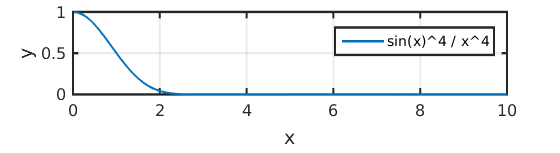
\includegraphics[width=0.49\textwidth]{b_integrand1.png}
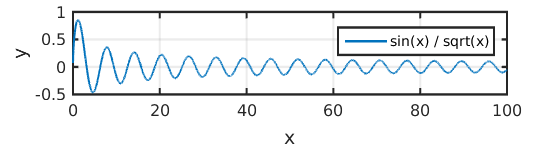
\includegraphics[width=0.49\textwidth]{b_integrand2.png}
\\[6pt]
\caption{Integrands for Problem B, parts (i) and (ii). Note the difference in how quickly the oscillations decay.}
\label{fig:b_integrands}
\end{center}
\end{figure}

\begin{figure}[h!]
\begin{center}
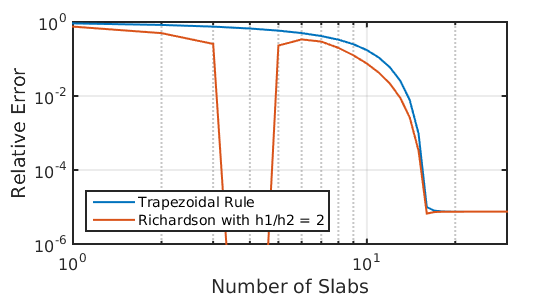
\includegraphics[width=0.49\textwidth]{b_err1.png}
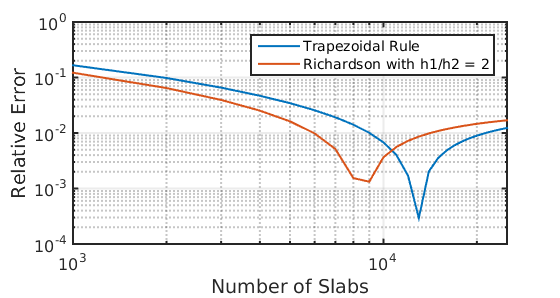
\includegraphics[width=0.49\textwidth]{b_err2.png}
\\[6pt]
\caption{Relative errors for Problem B, parts (i) and (ii), respectively.}
\label{fig:b_errs}
\end{center}
\end{figure}

\subsection{Problem C}

Results for Simpson's method applied to a two-dimensional integral are shown in Table \ref{t:c}.

\begin{table}[h!]
\centering
\begin{tabular}{l|lll}
Part & Exact & Calculated            & Error                      \\ \hline
(i)  & 46/3  & 15.333333333333332    & 1.15849359091320679264e-16 \\
(ii) & 365/3 & 1.216666666666667e+02 & 1.16801545604400043792e-16
\end{tabular}
\vspace{6pt}
\caption{Volume integration results for Problem C. Exact values are calculated by hand.}
\label{t:c}
\end{table}

\section{Discussion}

\subsection{Problem A}

In problem A, we see that Simpson's method performs well on the given integrand with as few as $n=10$ slabs used. Doubling the number of slabs reduces the error in both cases, for $n=10$ and $n=100$ slabs.

Note that for $n = \{100, 200\}$, the relative error does not change past $\bigo(10^{-16})$, because machine precision has been reached. Thus, is is no surprise that Richardson extrapolation fails to improve the $n=\{100,200\}$ estimate of the integral.

It is more surprising that Richardson extrapolation fails to improve upon the $n=20$ data when combined with the $n=10$ data. Its relative error is higher than that for $n=20$, suggesting that Richardson extrapolation is not always guaranteed to work. I posit that this has to do with the concavity of the function we are integrating. It looks like a bell curve, essentially, and it would seem that depending on the number of slabs used, the extrapolation method could overshoot, especially since it has so few slabs in this instance.

\subsection{Problem B}

In problem B, the integration scheme works perfectly for equation \eqref{eq:b}(i). As shown in Figure \ref{fig:b_errs}, the relative error of the trapezoidal method drops until the integration limit prevents any further increase in accuracy beyond $\sim 10^{-4}$. Richardson extrapolation outperforms the trapezoidal rule in this case as well. It takes slightly under 30 slabs to reduce the error below $10^{-4}$ in this scenario.

Integration is much more difficult for equation \eqref{eq:b}(ii), due to the slow rate of convergence as $x \rightarrow \infty$. Even though 300 periods were used for the domain of integration, and up to 20,000 integration points, we are still unable to attain a relative error under $10^{-4}$. Richardson extrapolation again is superior to the trapezoidal rule. This emphasizes the fact that some functions are easier to integrate than others.

\subsection{Problem C}

As shown in Table \ref{t:c}, both integrals were calculated exactly using Simpson's rule with a single two-dimensional slab of dimension $2h \times 2k$ (nine grid points). This is likely due to the face that both integrands are polynomial functions of order no higher than $3$ in either variable. Since Simpson's method has a global accuracy of $\bigo(10^{4})$, it is able to represent polynomials of degree $3$ and lower exactly. Thus, it is able to use the minimum possible number of grid points to exactly calculate the integrals provided.

\section{References}

No external references were used other than the course notes for this assignment.

\section*{Appendix: MATLAB Code}
The following code listings generate all figures presented in this homework assignment.

\includecode{Homework_1_Driver.m}
\includecode{RelErr.m}
\includecode{Problem_A.m}
\includecode{Simpsons.m}
\includecode{Problem_B.m}
\includecode{Trapezoidal_Inf.m}
\includecode{Problem_C.m}
\includecode{Simpsons_2D.m}
\includecode{Set_Default_Plot_Properties.m}
\includecode{Dashes.m}



%%
%% DOCUMENT END
%%
\end{document}
